\documentclass{ximera}

\title{Theory}
\author{Mila Vervoort}
\license{CC: 0}         % replace with an appropriate license, or set it in xmPreamble

\begin{document}
\begin{abstract}
    Samenvatting van de theorie over ideale homogene reactoren onder isotherme voorwaarden.
\end{abstract}
\maketitle
\label{xim:theory}

In hoofdstuk 3 'Ontwerp van homogene reaktoren onder isotherme werkingsvoorwaarden' werd gezien hoe door het opstellen van de stofbalans de nodige ontwerpvergelijkingen bekomen kunnen worden. 

Een stofbalans is van de volgende vorm: 
\[
\text{Accumulation} = \text{In} - \text{Uit} + \text{Vorming} - \text{Verbruik}
\]
In formulevorm:
\[
\frac{dN_A}{dt} = F_{A,in} - F_{A,out} + R_A V
\]
waar:
\begin{itemize}
\item $N_A$ = aantal mol van component A in de reactor
\item $F_{A,in}$ = molstroom van A naar binnen
\item $F_{A,out}$ = molstroom van A naar buiten
\item $R_A$ = reactiesnelheid van A (mol/(m$^3$s))
\item $V$ = reactorvolume
\end{itemize}

\begin{remark}
Monotoon stijgende kinetica

We veronderstellen een monotoom stijgende kinitiek in het vervolg van de theorie.
Voor een irreversibele reactie met monotoon stijgende kinetica geldt:

\[
R_A = \frac{dC_A}{dt} = -k C_A^n
\]

waarbij:

\begin{itemize}
\item $n=1$ : eerste orde
\item $n=2$ : tweede orde
\item $n=3$ : derde orde
\item $\dots$
\end{itemize}

Hieruit volgt:

\[
-\frac{1}{R_A} = \frac{1}{k C_A^n}
\]

De onderstaande grafiek toont $-1/R_A$ als functie van $C_A$
voor verschillende waarden van $n$. 

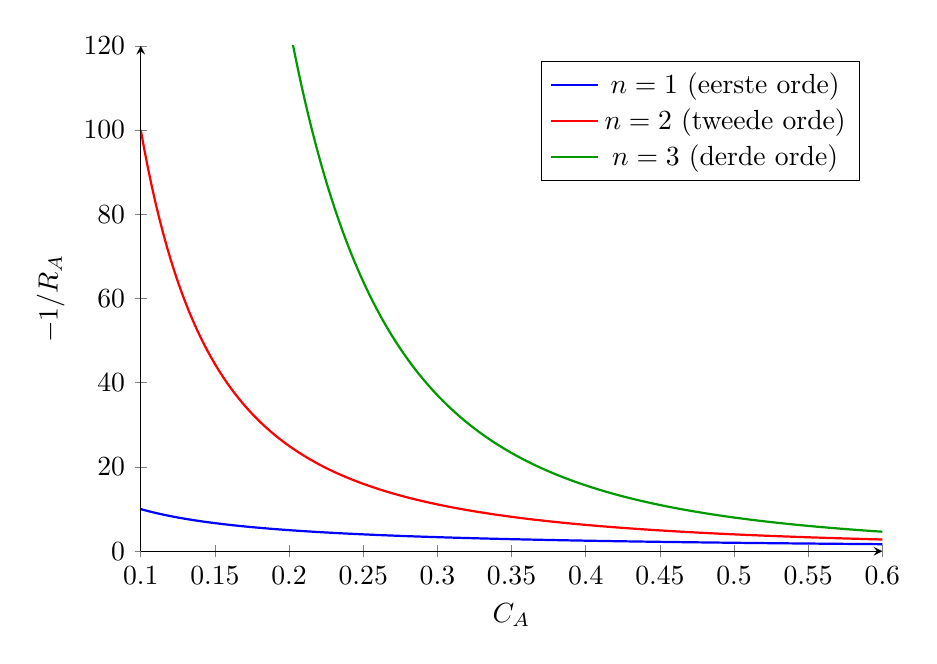
\begin{tikzpicture}
\begin{axis}[
    xlabel={$C_A$},
    ylabel={$-1/R_A$},
    domain=0.1:0.6,
    samples=200,
    axis lines=left,
    width=11cm,
    height=8cm,
    legend pos=north east,
    ymin=0,
    ymax=120,
]

% n = 1
\addplot[blue, thick] {1/x};
\addlegendentry{$n=1$ (eerste orde)}

% n = 2
\addplot[red, thick] {1/(x^2)};
\addlegendentry{$n=2$ (tweede orde)}

% n = 3
\addplot[green!60!black, thick] {1/(x^3)};
\addlegendentry{$n=3$ (derde orde)}

\end{axis}
\end{tikzpicture}
\end{remark}

\section*{1. Batch reactor}

\subsection*{Algemene massabalans}

In een batch reactor is er geen in- of uitstroom:

\[
\frac{dN_A}{dt} = r_A V
\]

Aangezien $N_A = N_{A0}(1-X_A)$:

\[
\boxed{
\frac{dX_A}{dt} = \frac{-r_A}{C_{A0}}
}
\]

\[
t = \int_0^{X_A} \frac{C_{A0}}{-r_A}\, dX_A
\]

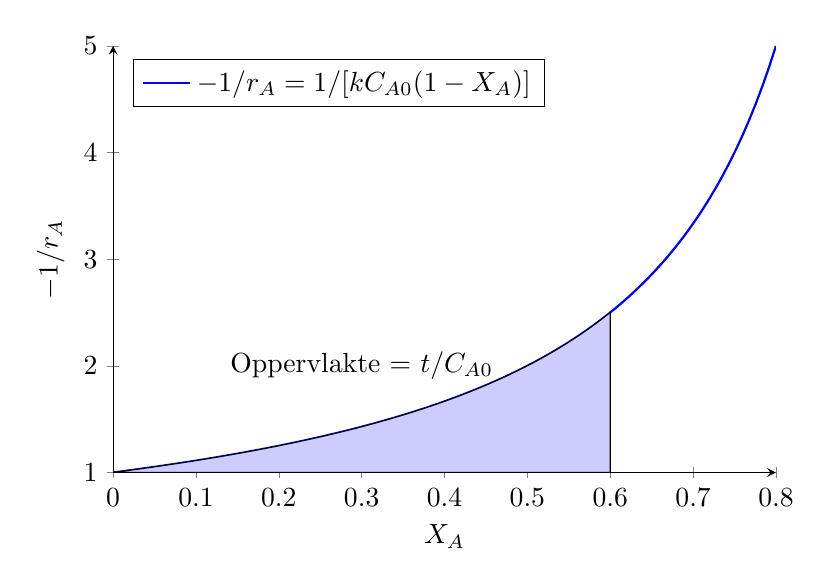
\begin{tikzpicture}
\begin{axis}[
    xlabel={$X_A$},
    ylabel={$-1/r_A$},
    domain=0:0.8,
    samples=100,
    axis lines=left,
    width=10cm,
    height=7cm,
    legend pos=north west,
]
\addplot[blue, thick] {1/(1-x)};
\addlegendentry{$-1/r_A = 1/[kC_{A0}(1-X_A)]$}

\addplot[
    domain=0:0.6,
    fill=blue!20
] {1/(1-x)} \closedcycle;

\draw[dashed] (axis cs:0.6,0) -- (axis cs:0.6,{1/(1-0.6)});
\node at (axis cs:0.3,2) {Oppervlakte = $t/C_{A0}$};

\end{axis}
\end{tikzpicture}

Bij constante densiteit:

\[
\boxed{
\frac{dC_A}{dt} = r_A
}
\]

\[
t = \int_{C_{A0}}^{C_A} \frac{dC_A}{r_A}
\]

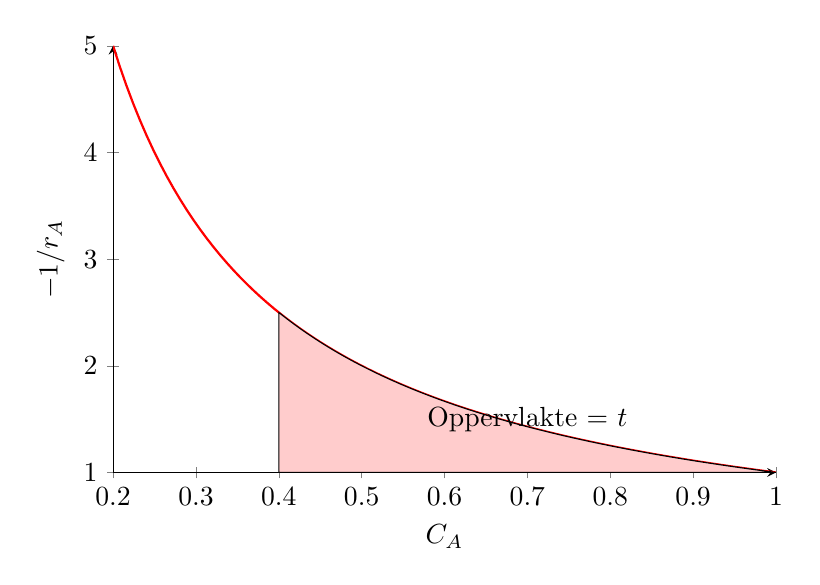
\begin{tikzpicture}
\begin{axis}[
    xlabel={$C_A$},
    ylabel={$-1/r_A$},
    domain=0.2:1,
    samples=100,
    axis lines=left,
    width=10cm,
    height=7cm,
]
\addplot[red, thick] {1/x};

\addplot[
    domain=0.4:1,
    fill=red!20
] {1/x} \closedcycle;

\node at (axis cs:0.7,1.5) {Oppervlakte = $t$};

\end{axis}
\end{tikzpicture}

 
\section*{1. Batch Reactor}

In een batch reactor is er geen in- of uitstroom (\(F_{A,in} = F_{A,out} = 0\)):

\[
\frac{dN_A}{dt} = R_A V
\]

Aanname dat het volume V constant blijft:

\[
\frac{dC_A}{dt} = R_A
\]


Om de tijd \(t\) te berekenen die nodig is om van een initiële concentratie \(C_{A0}\) naar \(C_A\) te gaan, integreren we:

\[
\frac{dC_A}{dt} = R_A(C_A)
\]

\[
\int_{t=0}^{t} dt = \int_{C_{A0}}^{C_A} \frac{dC_A}{R_A(C_A)}
\]

\[
t = \int_{C_A}^{C_{A0}} \frac{dC_A}{-R_A(C_A)}
\]

\begin{image}
\begin{tikzpicture}
\begin{axis}[
    domain=0:0.95,
    samples=200,
    xmin=0, xmax=1,
    ymin=0, ymax=12,
    axis lines=left,
    xlabel={$X_A$},
    ylabel={$\frac{1}{-r_A}$},
]

% parameters
\addplot[ultra thick, blue]
{1/(1*(1-x))};

\end{axis}
\end{tikzpicture}
\end{image}

\begin{image}
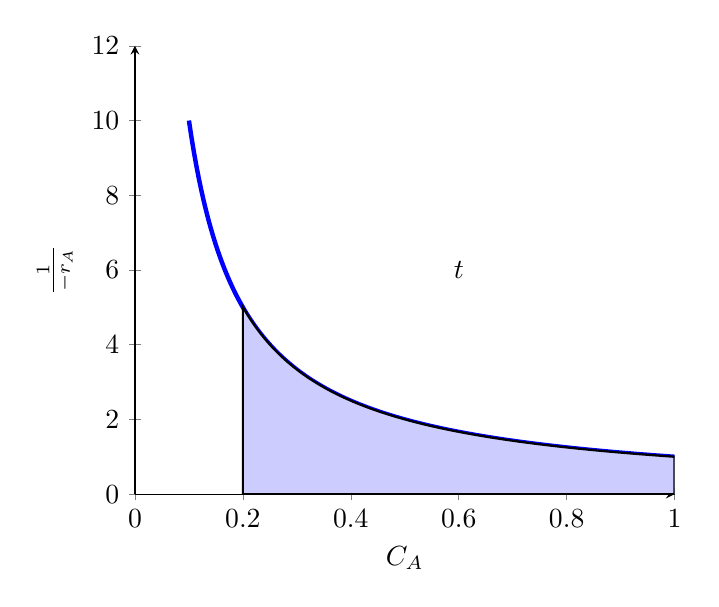
\begin{tikzpicture}
\begin{axis}[
    domain=0.1:1,       % x loopt van 0 tot C_A0
    samples=200,
    xmin=0, xmax=1,
    ymin=0, ymax=12,
    axis lines=left,
    xlabel={$C_A$},
    ylabel={$\frac{1}{-r_A}$},
]

% parameters
\def\k{1}   % snelheidsconstante

% plot de curve
\addplot[ultra thick, blue] {1/(\k*x)};

% arceer het gebied tussen C_A_end en C_A0
\addplot [
    thick,
    fill=blue!20,
    domain=0.2:1,   % van C_A,e tot C_A0
    samples=100
] {1/(\k*x)} \closedcycle;

% Voeg een t label toe in het gearceerde gebied
\node at (axis cs:0.6,6) {$t$};

\end{axis}
\end{tikzpicture}
\end{image}

\textbf{Voorbeeld eerste orde reactie:} \(R_A = -k C_A\)

\[
\frac{dC_A}{dt} = -k C_A \quad \Rightarrow \quad \int_{C_{A0}}^{C_A} \frac{dC_A}{-k C_A} = \int_0^t dt
\]

\[
t = \frac{1}{k} \ln \frac{C_{A0}}{C_A}
\]

\begin{image}
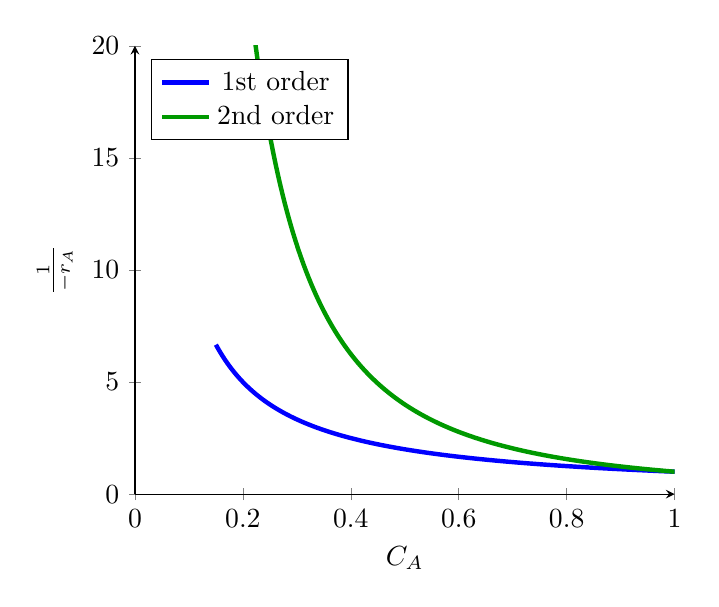
\begin{tikzpicture}
\begin{axis}[
    domain=0.15:1,
    samples=200,
    xmin=0, xmax=1,
    ymin=0, ymax=20,
    axis lines=left,
    xlabel={$C_A$},
    ylabel={$\frac{1}{-r_A}$},
    legend pos=north west,
]

\addplot[ultra thick, blue] {1/x};
\addlegendentry{1st order}

\addplot[ultra thick, green!60!black] {1/(x^2)};
\addlegendentry{2nd order}

\end{axis}
\end{tikzpicture}
\end{image}

\begin{image}
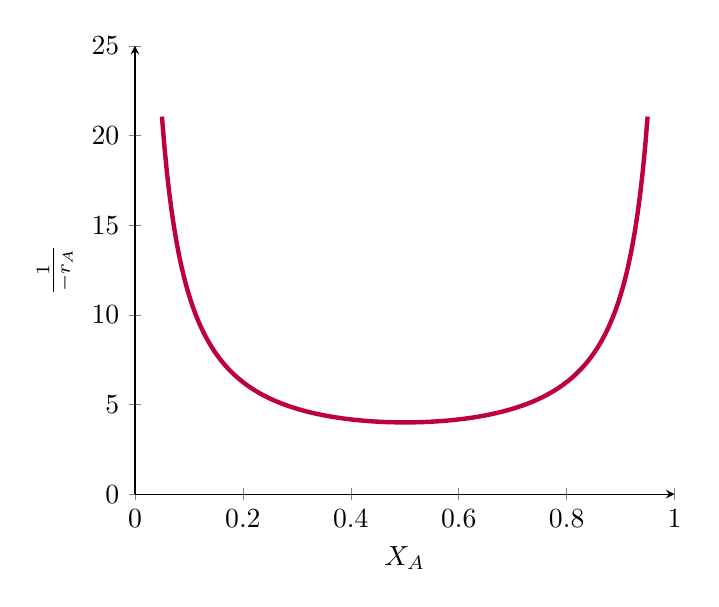
\begin{tikzpicture}
\begin{axis}[
    domain=0.05:0.95,
    samples=200,
    xmin=0, xmax=1,
    ymin=0, ymax=25,
    axis lines=left,
    xlabel={$X_A$},
    ylabel={$\frac{1}{-r_A}$},
]

\addplot[ultra thick, purple]
{1/(x*(1-x))};

\end{axis}
\end{tikzpicture}
\end{image}

\section*{2. CSTR (Continuous Stirred Tank Reactor)}

In een CSTR met constante volumestroom \(Q\) geldt bij stationaire toestand (\(\frac{dN_A}{dt} = 0\)):

\[
F_{A,in} - F_{A,out} + R_A V = 0
\]

Invullen van \(F_A = C_A Q\) geeft:

\[
Q C_{A,in} - Q C_{A,out} + R_A V = 0
\]

of herschikt:

\[
C_{A,out} = C_{A,in} + \frac{R_A V}{Q}
\]

\textbf{Uitleg:} In een goed gemengde CSTR is de concentratie overal uniform. De uitstroomconcentratie wordt bepaald door de balans tussen toevoer en reactie.

\section*{3. PFR (Plug Flow Reactor)}

In een PFR verandert de concentratie langs de reactorlengte \(x\). De stofbalans over een klein segment \(dx\) is:

\[
F_A(x) - F_A(x+dx) + R_A dV = 0
\]

Bij een constante volumestroom \(Q\) (bij vloeistoffen):

\[
Q \frac{dC_A}{dx} = R_A
\]

Met \(dV = A dx\) (doorsnede \(A\)):

\[
\frac{dC_A}{dx} = \frac{R_A}{Q}
\]

\textbf{Uitleg:} In een PFR stroomt het reactiemengsel plug-gewijs; er is geen menging in de lengterichting. De concentratie verandert continu langs de reactor.

\section*{Samenvatting}

\begin{tabular}{|l|c|c|}
    \hline
    \textbf{Reactor Type} & \textbf{Stofbalans} & \textbf{Kernidee}\\
    \hline
    Batch & $\frac{dC_A}{dt} = R_A$ & Geen in-/uitstroom, alleen reactie\\
    CSTR & $Q C_{A,in} - Q C_{A,out} + R_A V = 0$ & Goed gemengd, stationaire toestand\\
    PFR & $\frac{dC_A}{dx} = \frac{R_A}{Q}$ & Concentratie verandert langs de lengte, plug-flow\\
    \hline
\end{tabular}


\end{document}